
\documentclass[a4paper,czech,czech,openright,cleardoubleempty,BCOR10mm,DIV11]{scrreprt}
\usepackage[T1]{fontenc}
\usepackage[utf8]{inputenc}
\usepackage{array}
\usepackage{longtable}
\usepackage{varioref}
\usepackage{wrapfig}
\usepackage{fancybox}
\usepackage{calc}
\usepackage{framed}
\usepackage{url}
\usepackage{graphicx}
\usepackage{placeins} %floatbarrier \FloatBarrier
%\usepackage{listing}
\usepackage{pdfpages}

\makeatletter

\usepackage[font=small,labelfont=bf]{caption} %captiony

%%%%%%%%%%%%%%%%%%%%%%%%%%%%%% LyX specific LaTeX coěmmands.
\providecommand{\LyX}{L\kern-.1667em\lower.25em\hbox{Y}\kern-.125emX\@}
\newcommand{\lyxline}[1][1pt]{%
  \par\noindent%
  \rule[.5ex]{\linewidth}{#1}\par}
\newcommand{\noun}[1]{\textsc{#1}}
%% Special footnote code from the package 'stblftnt.sty'
%% Author: Robin Fairbairns -- Last revised Dec 13 1996
\let\SF@@footnote\footnote
\def\footnote{\ifx\protect\@typeset@protect
    \expandafter\SF@@footnote
  \else
    \expandafter\SF@gobble@opt
  \fi
}

\renewcommand{\baselinestretch}{1.2} %radkovani s

\expandafter\def\csname SF@gobble@opt \endcsname{\@ifnextchar[%]
  \SF@gobble@twobracket
  \@gobble
}
\edef\SF@gobble@opt{\noexpand\protect
  \expandafter\noexpand\csname SF@gobble@opt \endcsname}
\def\SF@gobble@twobracket[#1]#2{}
%% Because html converters don't know tabularnewline
\providecommand{\tabularnewline}{\\}

%%%%%%%%%%%%%%%%%%%%%%%%%%%%%% Textclass specific LaTeX commands.
\newenvironment{lyxcode}
{\begin{list}{}{
\setlength{\rightmargin}{\leftmargin}
\setlength{\listparindent}{0pt}% needed for AMS classes
\raggedright
\setlength{\itemsep}{0pt}
\setlength{\parsep}{0pt}
\normalfont\ttfamily}%
 \item[]}
{\end{list}}

%<-------------------------------společná nastavení------------------------------>
\usepackage[czech]{babel} % localize labels to czech (Obsah, Kapitola, Literatura atp.)
\usepackage[]{hyperref} %odkazy v  pdf jsou klikací s barevnými rámečky
\usepackage[numbers,sort&compress]{natbib} %balíček pro citace literatury  
\usepackage{hypernat}%interakce mezi hyperref a natbib
\hypersetup{   % some PDF metadata
pdftitle={Platforma Vert.x},%   
pdfauthor={Michael Kutý},%  
pdfsubject={},%   
pdfkeywords={Vert.x, D3.js, MongoDB}%                             
}
\usepackage{multicol}



%<------------------------------------font settings----------------------------------------->
%\usepackage{packages/bc-latinmodern}
%\usepackage{packages/bc-times}
\usepackage{packages/bc-palatino}
%\usepackage{packages/bc-iwona}
%\usepackage{packages/bc-helvetika}


%<------------------------------headings stránek------------------------------------>
%\usepackage{packages/bc-headings}
\usepackage{packages/bc-fancyhdr}

%\usepackage{packages/bc-neueskapitel}
%\usepackage{packages/bc-fancychap}

\makeatother

\usepackage{babel}

%<------------------------------snippets settings------------------------------------>
\usepackage{listing}
\usepackage{listings}
\usepackage{color}

\renewcommand*{\lstlistingname}{Ukázka kódu} % labeling
\renewcommand*{\lstlistlistingname}{Seznam ukázek kódu} % labeling

\definecolor{dkgreen}{rgb}{0,0.6,0}
\definecolor{gray}{rgb}{0.5,0.5,0.5}
\definecolor{mauve}{rgb}{0.58,0,0.82}

% syntax highlight for Java languae %
\lstset{
  %frame=r,
  captionpos=b,
  language=Java,
  aboveskip=3mm,
  belowskip=3mm,
  xleftmargin=0.2mm,
  showstringspaces=false,
  columns=flexible,
  basicstyle={\small\ttfamily},
  numbers=none,
  numberstyle=\tiny\color{gray},
  keywordstyle=\color{blue},
  commentstyle=\color{dkgreen},
  stringstyle=\color{mauve},
  breaklines=true,
  breakatwhitespace=true,
  tabsize=3,
    inputencoding=utf8,
    extendedchars=true,
    literate=%
    {á}{{\'a}}1
    {č}{{\v{c}}}1
    {ď}{{\v{d}}}1
    {é}{{\'e}}1
    {ě}{{\v{e}}}1
    {í}{{\'i}}1
    {ň}{{\v{n}}}1
    {ó}{{\'o}}1
    {ř}{{\v{r}}}1
    {š}{{\v{s}}}1
    {ť}{{\v{t}}}1
    {ú}{{\'u}}1
    {ů}{{\r{u}}}1
    {ý}{{\'y}}1
    {ž}{{\v{z}}}1
    {Á}{{\'A}}1
    {Č}{{\v{C}}}1
    {Ď}{{\v{D}}}1
    {É}{{\'E}}1
    {Ě}{{\v{E}}}1
    {Í}{{\'I}}1
    {Ň}{{\v{N}}}1
    {Ó}{{\'O}}1
    {Ř}{{\v{R}}}1
    {Š}{{\v{S}}}1
    {Ť}{{\v{T}}}1
    {Ú}{{\'U}}1
    {Ů}{{\r{U}}}1
    {Ý}{{\'Y}}1
    {Ž}{{\v{Z}}}1
}

\begin{document}

\cleardoublepage{}~\thispagestyle{empty}\begin{center}\pagenumbering{roman}\vspace{10mm}


\textsf{\textsc{\noun{\LARGE Univerzita Hradec Králové}}}\\
\vspace{0.5em}
\textsc{\noun{\LARGE Fakulta informatiky a managementu}}\\
\vspace*{1em}
\textsf{\textsc{\noun{\Large katedra informatiky a kvantitativních metod }}}

\vspace{15mm}


\includegraphics[width=0.4\textwidth]{logos/uhk}

\vspace{15mm}


\textsf{\huge BAKALÁŘSKÁ / DIPLOMOVÁ PRÁCE}{\huge \par}

\vspace{15mm}


\textsf{\LARGE Dummy Name Foo Bar}{\LARGE \par}

\vspace{10mm}


\end{center} 

\vspace*{\fill}


\vspace{10mm}

\begin{description}
\item [{{\large Autor:}}] \noindent \textsf{\large Foo Bar}{\large \par}
\item [{{\large Vedoucí~práce:}}] \noindent \textsf{\large Bar Foo}{\large \hfill{}}\textsf{\large Moon, 2050}{\large{}
}{\large \par}
\end{description}
\clearpage{}

%{\small \thispagestyle{plain}\addcontentsline{toc}{chapter}{Abstrakt} }{\small \par}

\newpage{}\thispagestyle{plain}

{\small \setcounter{page}{3} % nastavení číslování stránek
\ }{\small \par}

\noindent {\small \vfill{}
% set next text to bottom
~}{\small \par}

\subsubsection{Prohlášení}

\noindent {\small Prohlašuji, že jsem bakalářskou práci vypracoval samostatně a uvedl jsem všechny použité prameny a literaturu.}{\small \par}

{\small \bigskip{}
}\noindent {\small{} V Hradci Králové dne \today\hspace{\fill}Foo Bar}\\
{\small{} % doplňte patřičné datum, jméno a příjmení
}{\small \par}

\clearpage{}

\newpage{}\thispagestyle{plain}

{\small %\setcounter{page}{3} % nastavení číslování stránek
\ }{\small \par}

\noindent {\small \vfill{}
 % set next text to bottom
~}{\small \par}

\subsubsection{Poděkování}

\noindent {\small Lorem ipsum dolor sit amet, consectetuer adipiscing elit. Aenean placerat. Duis pulvinar. Maecenas lorem. Mauris tincidunt sem sed arcu. Nemo enim ipsam voluptatem quia voluptas sit aspernatur aut odit aut fugit, sed quia consequuntur magni dolores eos qui ratione voluptatem sequi nesciunt. \newpage{}}{\small \par}

\clearpage{}

\newpage{}\thispagestyle{plain}

\noindent {\small \vfill{}
~}{\small \par}

\subsubsection{Anotace}

Lorem ipsum dolor sit amet, consectetuer adipiscing elit. Aenean placerat. Duis pulvinar. Maecenas lorem. Mauris tincidunt sem sed arcu. Nemo enim ipsam voluptatem quia voluptas sit aspernatur aut odit aut fugit, sed quia consequuntur magni dolores eos qui ratione voluptatem sequi nesciunt. Phasellus rhoncus. Praesent vitae arcu tempor neque lacinia pretium. Mauris suscipit, ligula sit amet pharetra semper, nibh ante cursus purus, vel sagittis velit mauris vel metus. Etiam posuere lacus quis dolor. Curabitur bibendum justo non orci. Praesent in mauris eu tortor porttitor accumsan. Nullam lectus justo, vulputate eget mollis sed, tempor sed magna. Donec quis nibh at felis congue commodo. Integer tempor. Maecenas libero.

\subsubsection{Annotation}

Lorem ipsum dolor sit amet, consectetuer adipiscing elit. Aenean placerat. Duis pulvinar. Maecenas lorem. Mauris tincidunt sem sed arcu. Nemo enim ipsam voluptatem quia voluptas sit aspernatur aut odit aut fugit, sed quia consequuntur magni dolores eos qui ratione voluptatem sequi nesciunt. Phasellus rhoncus. Praesent vitae arcu tempor neque lacinia pretium. Mauris suscipit, ligula sit amet pharetra semper, nibh ante cursus purus, vel sagittis velit mauris vel metus. Etiam posuere lacus quis dolor. Curabitur bibendum justo non orci. Praesent in mauris eu tortor porttitor accumsan. Nullam lectus justo, vulputate eget mollis sed, tempor sed magna. Donec quis nibh at felis congue commodo. Integer tempor. Maecenas libero.


\cleardoublepage{}

{\small %%%   place for the signature
%%%                                         *********
}{\small \par}

\cleardoublepage{}\thispagestyle{empty}{\small 

%\setcounter{secnumdepth}{3}
%\setcounter{tocdepth}{2}% depth of content

\tableofcontents{}% generated content
\cleardoublepage{}}{\small \par}

\pagenumbering{arabic}% start arabic pagination from 1 

\chapter{Example Chapter}


\begin{lstlisting}[caption=Some Java code with UTF-8 comments]
// žluťoučký kůň +ěščřžýáíé
import org.vertx.java.core.Handler;
import org.vertx.java.core.http.HttpServerRequest;
import org.vertx.java.platform.Verticle;

public class Server extends Verticle {
    public void start() {
        vertx.createHttpServer().requestHandler(new Handler<HttpServerRequest>() {
            public void handle(HttpServerRequest req) {
                String file = req.path().equals("/") ? "index.html" : req.path();
                req.response().sendFile("webroot/" + file);
            }
        }).listen(8080);
    }
}
\end{lstlisting}

\subsection{Interakce s Vert.x}\label{sub:interaction}

Lorem ipsum dolor sit amet, consectetuer adipiscing elit. Aenean placerat. Duis pulvinar. Maecenas lorem. Mauris tincidunt sem sed arcu. Nemo enim ipsam voluptatem quia voluptas sit aspernatur aut odit aut fugit, sed quia SSH\footnote{Secure Shell} magni dolores eos qui ratione voluptatem sequi nesciunt. Phasellus rhoncus. Praesent vitae arcu tempor neque lacinia pretium. Mauris suscipit, ligula sit amet pharetra semper, nibh ante cursus purus, vel sagittis velit mauris vel metus. Etiam posuere lacus quis dolor. Curabitur bibendum justo non orci. Praesent in mauris eu tortor porttitor accumsan. Nullam lectus justo, vulputate eget mollis sed, tempor sed magna. Donec quis nibh at felis congue commodo. Integer tempor. Maecenas libero.e.
\begin{figure}[h]
\begin{centering}
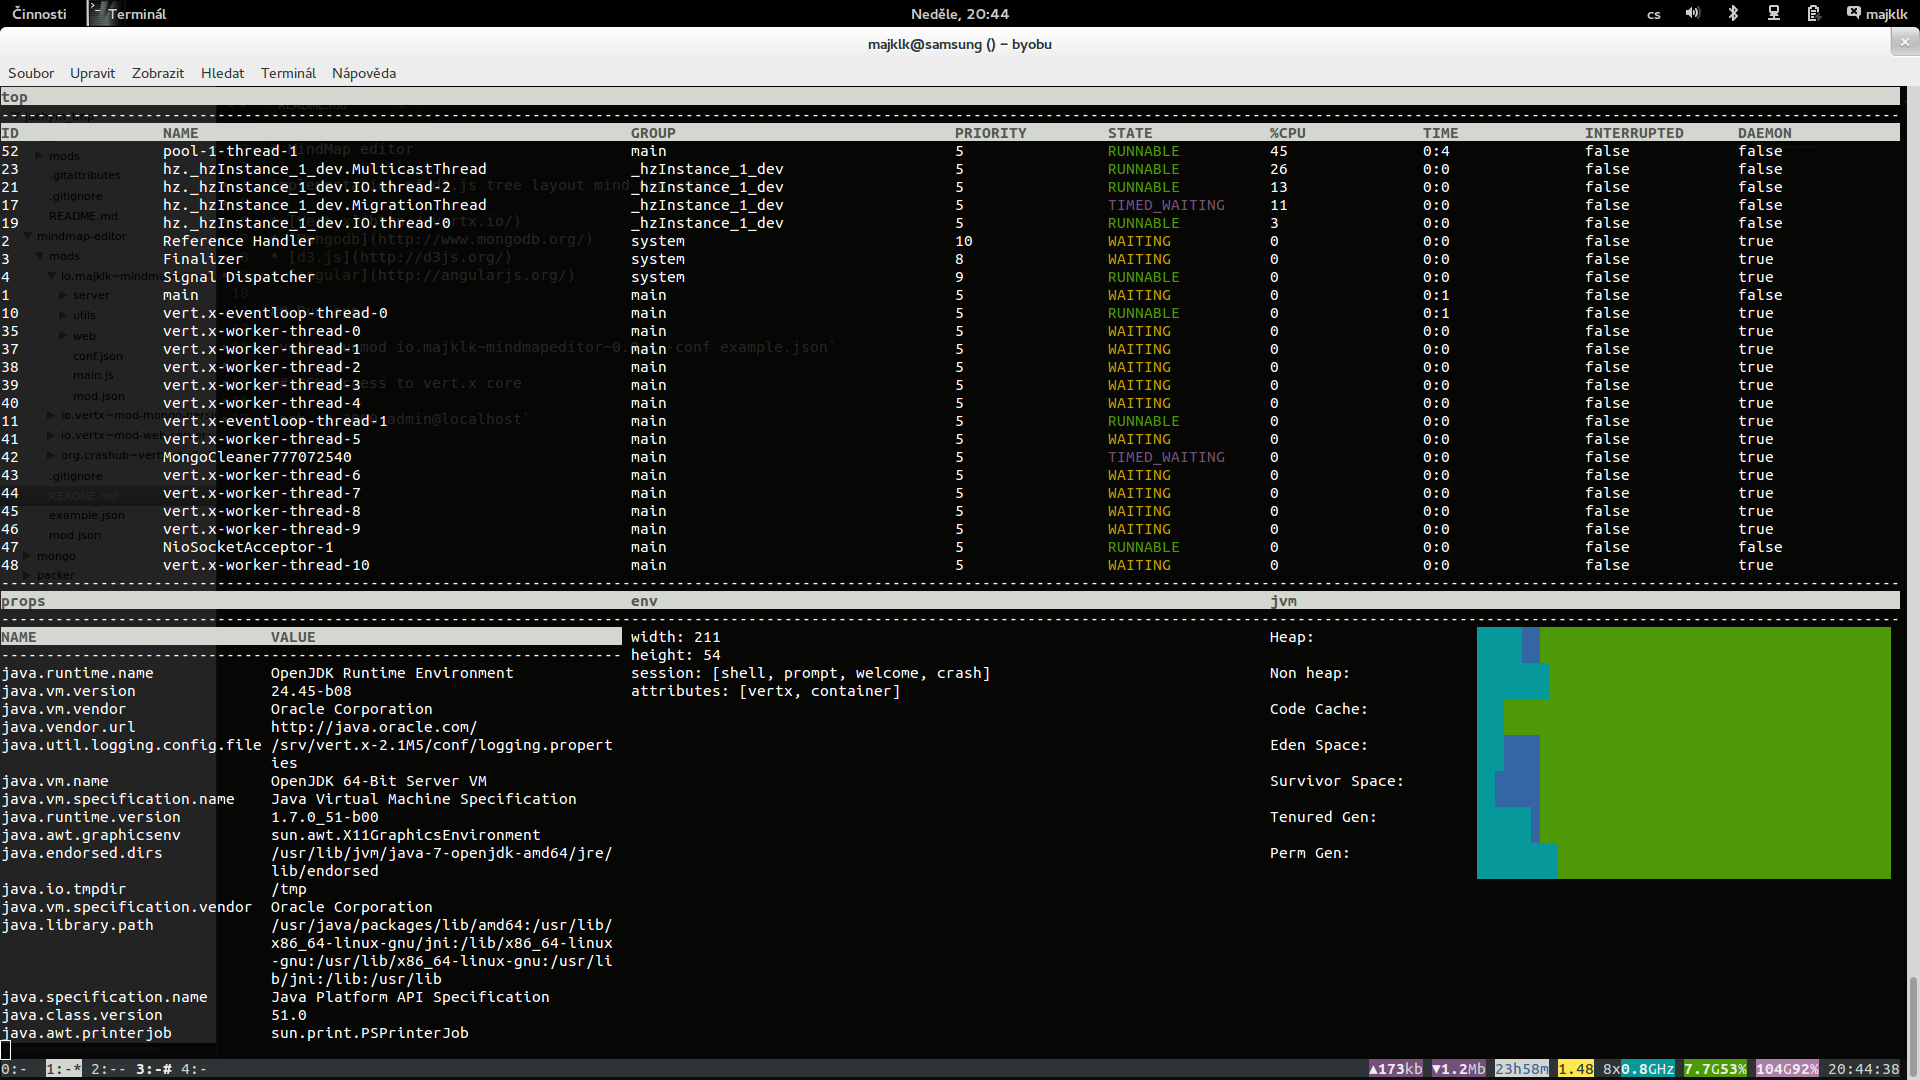
\includegraphics[scale=0.21]{images/real_interaction}
\par\end{centering}
\caption{Modul CrasHub Shell\label{fig:real_interaction}}
\end{figure}



%<------------------------------bibliography------------------------------------>
\begin{thebibliography}{10}

\bibitem{JAX}Kamali, Masoud \emph{The Winners of the JAX Innovation Awards 2014}
{[}online]. {[}cit. 2014-03-20]. Dostupný z WWW: \url{http://jax.de/awards2014/}

\end{thebibliography}

\cleardoublepage{}

\addcontentsline{toc}{part}{Přílohy}\thispagestyle{empty}  \renewcommand{\appendixname}{P\v{r}iloha}%%přílohy, číslování římskými
\part*{Přílohy} %% rename
\appendix
\chapter{Heat template Lbaas - HAproxy}

\begin{lstlisting}
heat_template_version: 2013-05-23
description: LBAAS Template
parameters:
  key_name:
    type: string
  instance_flavor:
    type: string
    description: Instance type for servers
    default: m1.small
    constraints:
      - allowed_values: [m1.tiny, m1.small, m1.medium, m1.large]
        description: instance_type must be a valid instance type
  instance_image:
    type: string
    description: Image name to use for the servers.
    default: ubuntu-14-04-x64
  public_net_id:
    type: string
    description: ID or name of public network for which floating IP addresses will be allocated
  router_name:
    type: string
    description: Name of router to be created
    default: test-router
  lb_name:
    type: string
    description: Name of balancer to be created
    default: test-lb
  public_net_name:
    type: string
    description: Name of public network to be created
    default: public-net
  public_net_cidr:
    type: string
    description: Public network address (CIDR notation)
    default: 10.10.20.0/24
  public_net_pool_start:
    type: string
    description: Start of public network IP address allocation pool
    default: 10.10.20.100
  public_net_pool_end:
    type: string
    description: End of public network IP address allocation pool
    default: 10.10.20.200
  private_net_name:
    type: string
    description: Name of private network to be created
    default: private-net
  private_net_cidr:
    type: string
    description: Private network address (CIDR notation)
    default: 10.10.10.0/24
  private_net_pool_start:
    type: string
    description: Start of private network IP address allocation pool
    default: 10.10.10.100
  private_net_pool_end:
    type: string
    description: End of private network IP address allocation pool
    default: 10.10.10.200
resources:
  http_security_group:
    type: OS::Neutron::SecurityGroup
    properties:
      name: http
      rules:
      - direction: ingress
        remote_mode: remote_ip_prefix
        remote_ip_prefix: 0.0.0.0/0
        port_range_min: 80
        port_range_max: 80
        protocol: tcp
  public_net:
    type: OS::Neutron::Net
    properties:
      admin_state_up: True
      name: { get_param: public_net_name }
      shared: False
  public_subnet:
    type: OS::Neutron::Subnet
    properties:
      allocation_pools:
      - start: { get_param: public_net_pool_start }
        end: { get_param: public_net_pool_end }
      cidr: { get_param: public_net_cidr }
      enable_dhcp: True
      ip_version: 4
      name: { get_param: public_net_name }
      network_id: { get_resource: public_net }
  private_net:
    type: OS::Neutron::Net
    properties:
      admin_state_up: True
      name: { get_param: private_net_name }
      shared: False
  private_subnet:
    type: OS::Neutron::Subnet
    properties:
      allocation_pools:
      - start: { get_param: private_net_pool_start }
        end: { get_param: private_net_pool_end }
      cidr: { get_param: private_net_cidr }
      enable_dhcp: True
      ip_version: 4
      name: { get_param: private_net_name }
      network_id: { get_resource: private_net }
  router:
    type: OS::Neutron::Router
    properties:
      name: { get_param: router_name }
      external_gateway_info:
        network: { get_param: public_net_id }
  router_interface:
    type: OS::Neutron::RouterInterface
    properties:
      router_id: { get_resource: router }
      subnet_id: { get_resource: private_subnet }
  lb_ping_healt_monitor:
    type: OS::Neutron::HealthMonitor
    properties:
      admin_state_up: True
      delay: 5
      max_retries: 1
      timeout: 5
      type: PING
  lb_pool:
    type: OS::Neutron::Pool
    properties:
      admin_state_up: True
      lb_method: ROUND_ROBIN
      name: { get_param: lb_name }
      protocol: HTTP
      monitors:
      - { get_resource: lb_ping_healt_monitor }
      subnet_id: { get_resource: private_subnet }
      vip:
        protocol_port: 80
#        address: { get_param: public_net_ip }
        admin_state_up: True
        subnet: { get_resource: public_subnet }
  instance_01:
    type: OS::Nova::Server
    properties:
      image: { get_param: instance_image }
      flavor: { get_param: instance_flavor }
      key_name: { get_param: key_name }
      name: test-web01
      networks:
      - network: { get_resource: private_net }
      security_groups:
      - default
      - { get_resource: http_security_group }
      user_data_format: RAW
      user_data: |
        #!/bin/bash -v
        apt-get install apache2 -yy
        echo "Instance 01" > /var/www/html/index.html
  lb_pool_member_instance_01:
    type: OS::Neutron::PoolMember
    properties:
      address: { get_attr: [ instance_01 , first_address ] }
      admin_state_up: True
      pool_id: { get_resource: lb_pool }
      protocol_port: 80
      weight: 1
  instance_02:
    type: OS::Nova::Server
    properties:
      image: { get_param: instance_image }
      flavor: { get_param: instance_flavor }
      key_name: { get_param: key_name }
      name: test-web02
      networks:
      - network: { get_resource: private_net }
      security_groups:
      - default
      - { get_resource: http_security_group }
      user_data_format: RAW
      user_data: |
        #!/bin/bash -v
        apt-get install apache2 -yy
        echo "Instance 02" > /var/www/html/index.html
  lb_pool_member_instance_02:
    type: OS::Neutron::PoolMember
    properties:
      address: { get_attr: [ instance_02 , first_address ] }
      admin_state_up: True
      pool_id: { get_resource: lb_pool }
      protocol_port: 80
      weight: 1
  lb:
    type: OS::Neutron::LoadBalancer
    properties:
      members:
      - { get_resource: instance_01 }
      - { get_resource: instance_02 }
      pool_id: { get_resource: lb_pool }
      protocol_port: 80
  lb_floating:
    type: OS::Neutron::FloatingIP
    properties:
      floating_network_id: {get_param: public_net_id}
      port_id: {get_attr: [lb_pool, vip, port_id]}
\end{lstlisting}

\chapter{Heat template FwaaS}



%<------------------------------external PDF------------------------------------>
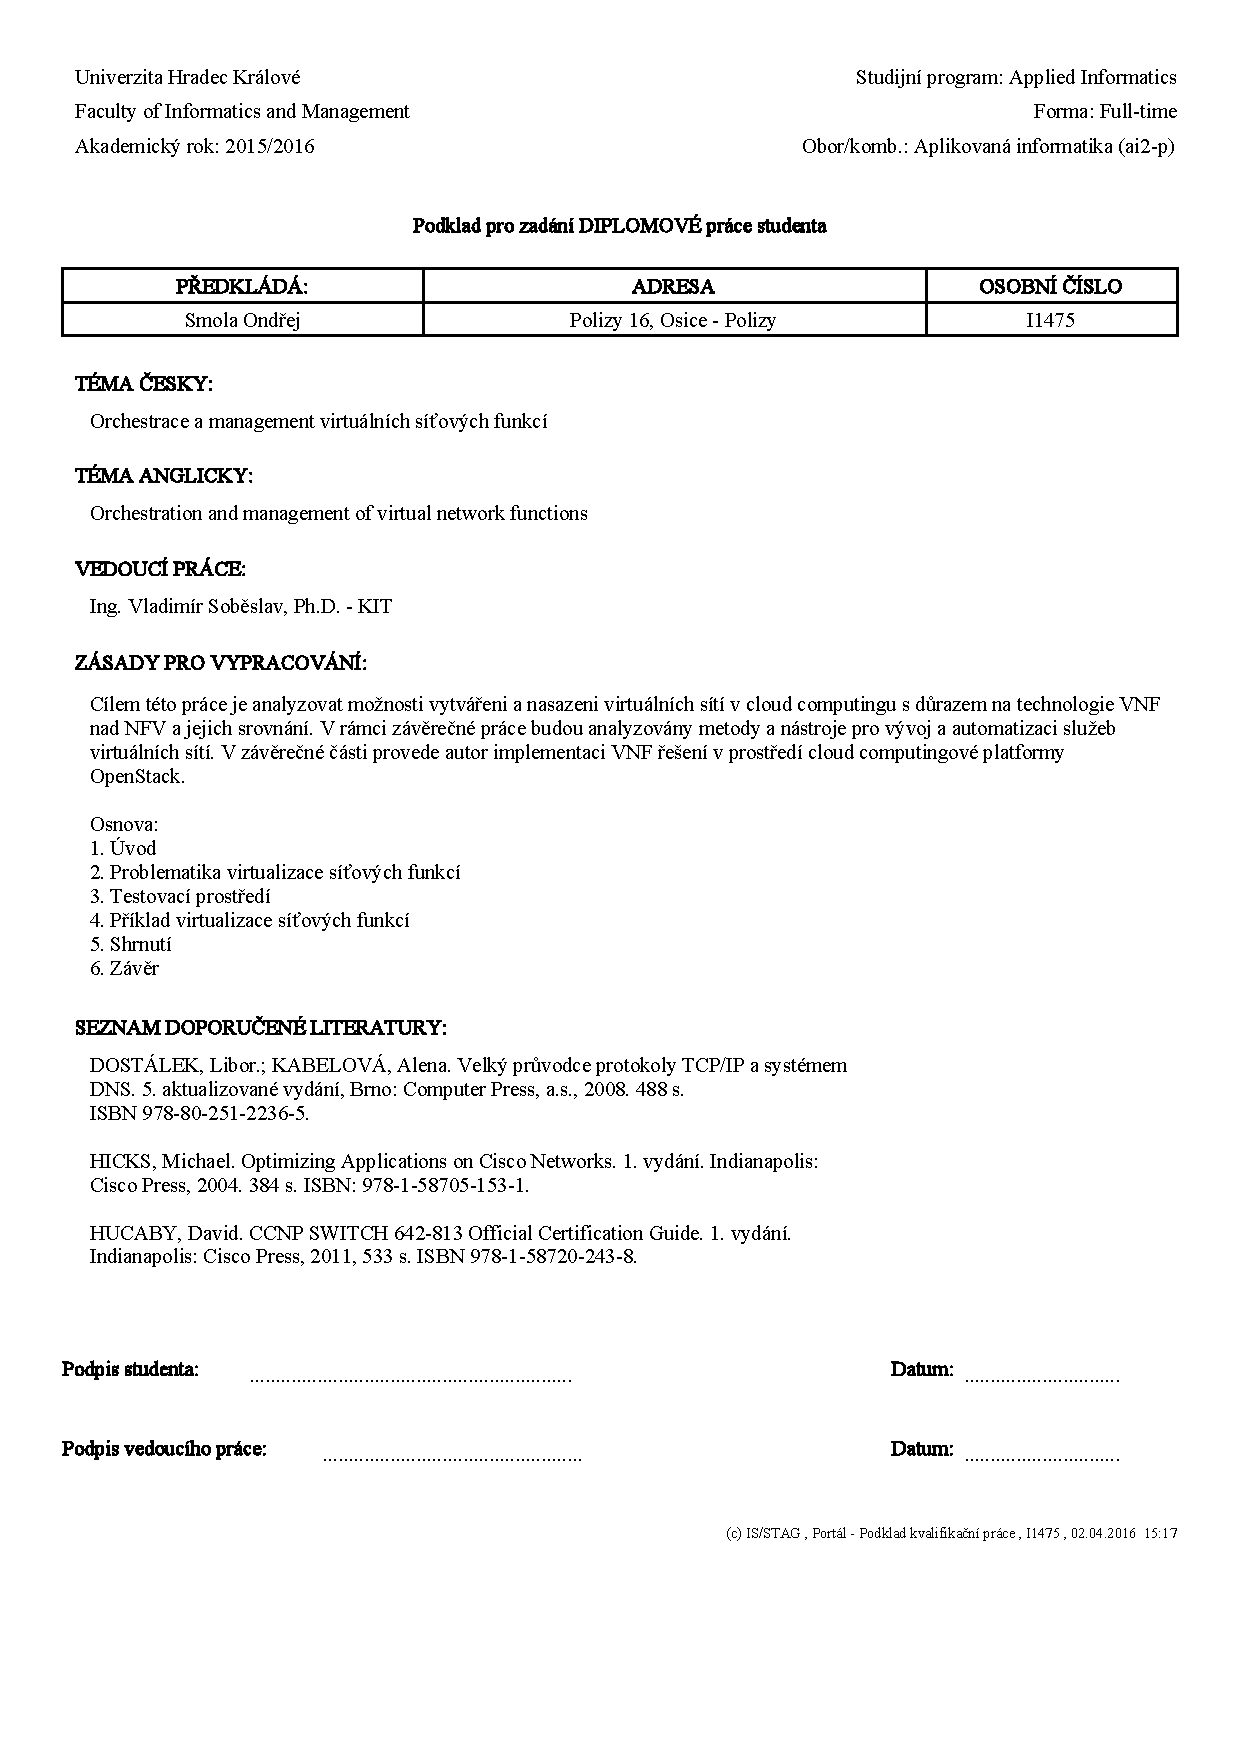
\includepdf[pages={1}]{zadani.pdf}

\end{document}
